\begin{figure}[htpb]
\centering\capstart{}
\subfloat[\(\pixel{f}\)]
{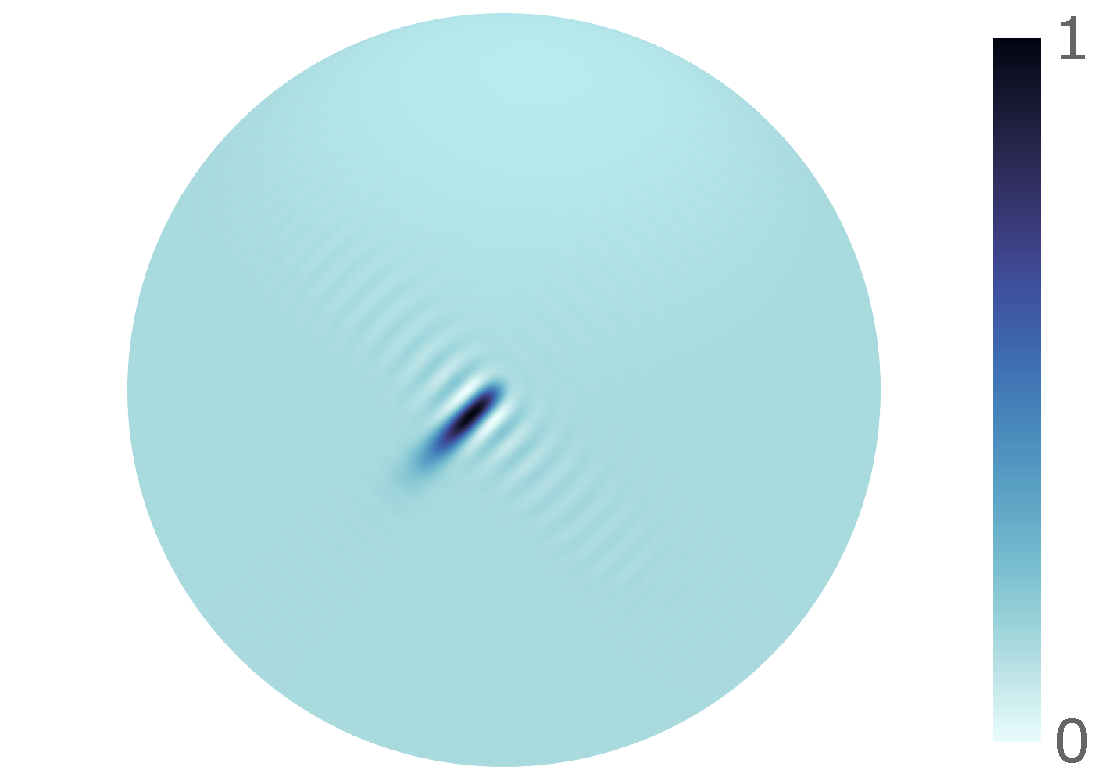
\includegraphics[trim={4 7 3 6},clip,width=.5\textwidth]{elongated_gaussian_1tsig10_1psig10_L128_res512_real_norm.pdf}}
    \hfill
    \subfloat[\(\pixel{(\rotation{(0,0,\pi/4)}f)}\)]
{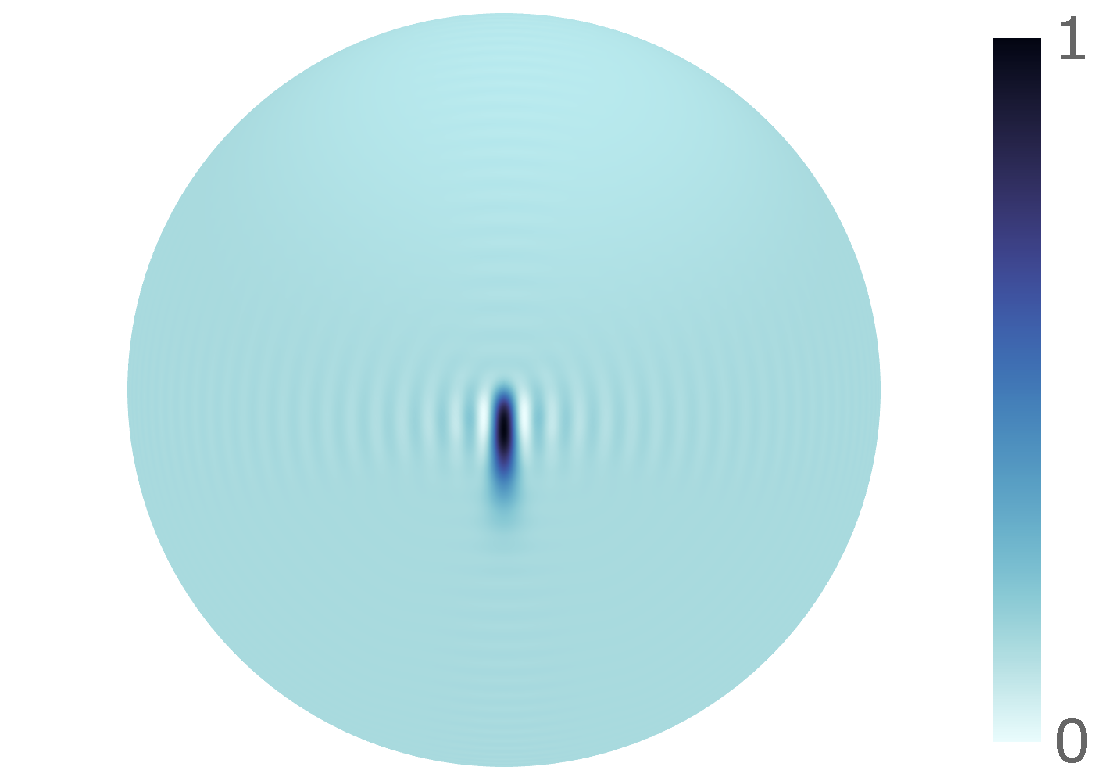
\includegraphics[trim={4 7 3 6},clip,width=.5\textwidth]{elongated_gaussian_1tsig10_1psig10_L128_rotate_alpha0_beta0_gamma1pi4_res512_real_norm.pdf}}
    \newline
    \subfloat[\(\pixel{(\rotation{(0,\pi/4,\pi/4)}f)}\)]
{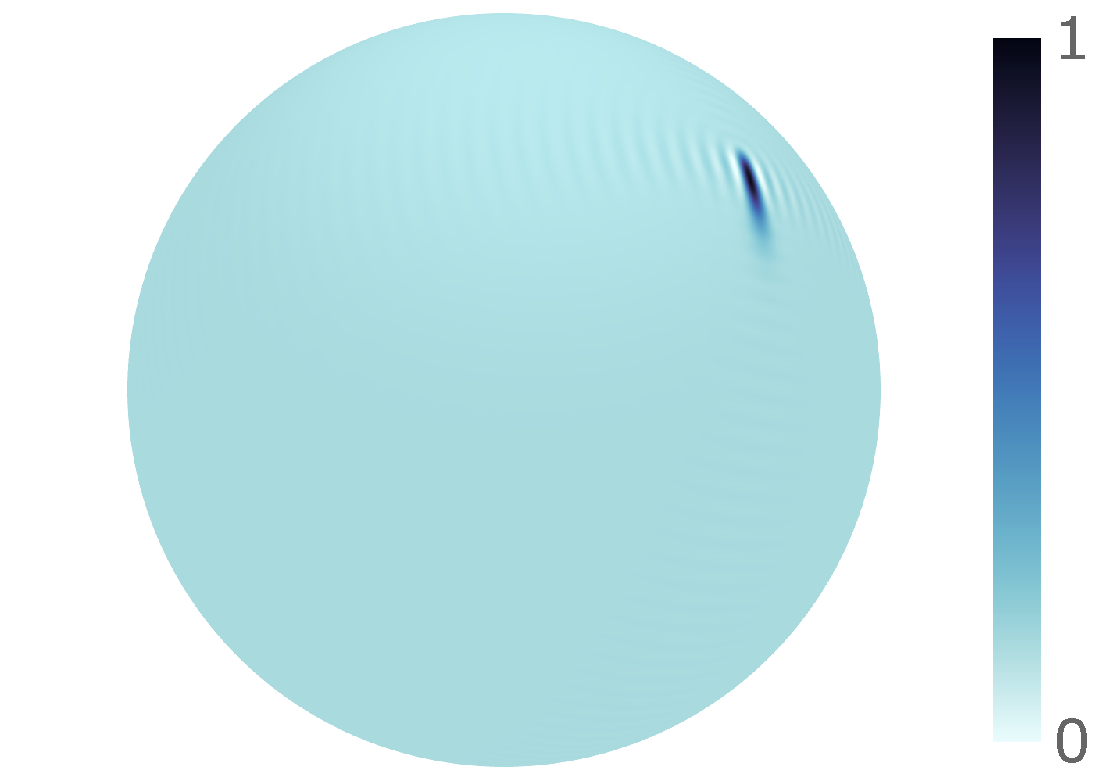
\includegraphics[trim={4 7 3 6},clip,width=.5\textwidth]{elongated_gaussian_1tsig10_1psig10_L128_rotate_alpha0_beta1pi4_gamma1pi4_res512_real_norm.pdf}}
    \hfill
    \subfloat[\(\pixel{(\rotation{(\pi/4,\pi/4,\pi/4)}f)}\)]
{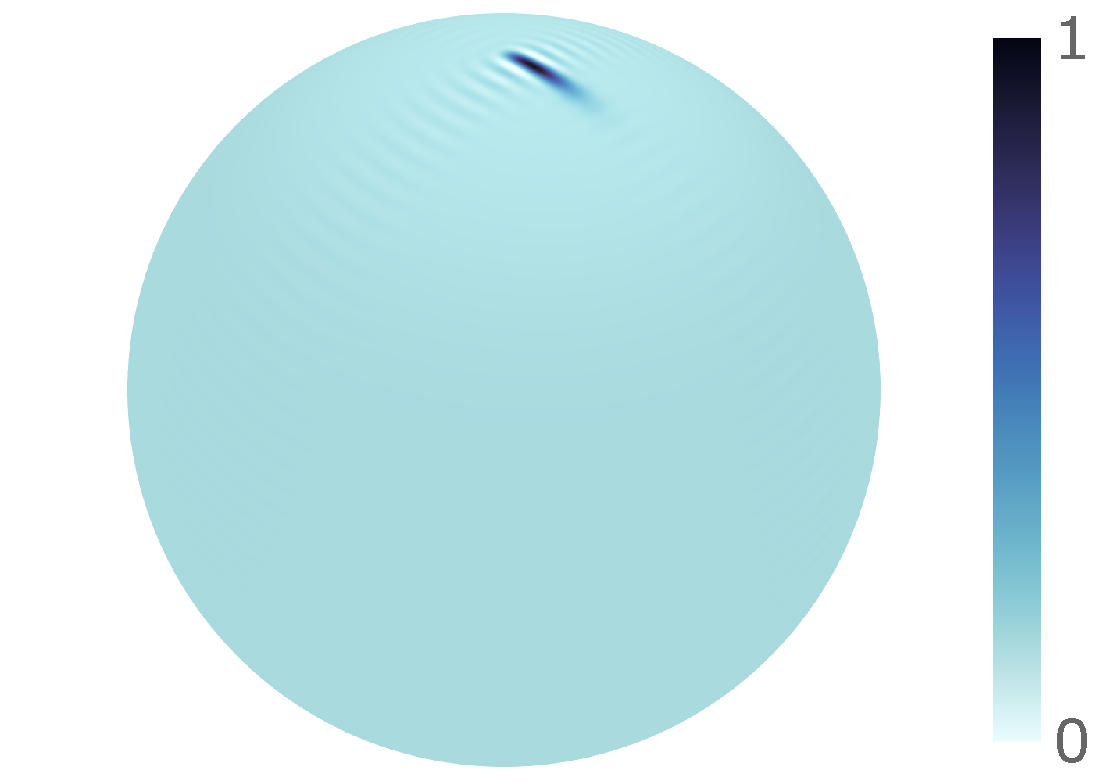
\includegraphics[trim={4 7 3 6},clip,width=.5\textwidth]{elongated_gaussian_1tsig10_1psig10_L128_rotate_alpha1pi4_beta1pi4_gamma1pi4_res512_real_norm.pdf}}
\caption[
A demonstration of the three-dimensional rotation
]{
Panel (a) presents a directional function on the north pole (bandlimited at \(L=128\)).
The effect of a three-dimensional rotation is then demonstrated in panels (b--d). % chktex 8
The kernel is first rotated \(\gamma=\frac{\pi}{4}\) about the \(z\)-axis --- which points out of the page --- resulting in panel (b).
Panel (b) is then rotated \(\beta=\frac{\pi}{4}\) about the \(y\)-axis --- which points from bottom-right to top-left --- to produce panel (c).
Finally, panel (c) is rotated \(\alpha=\frac{\pi}{4}\) about the original \(z\)-axis by \(\alpha=\frac{\pi}{4}\) producing panel (d).
Three-dimensional rotations are fully parameterised by the three Euler angles.
}\label{fig:chapter2_rotation_sphere}
\end{figure}
